\documentclass[xcolor=dvipsnames]{beamer}
\usepackage[T1]{fontenc}
\usepackage[utf8]{inputenc}
\usepackage[english,slovak]{babel}

\usepackage{amsmath}
\usepackage{amsthm}
\usetheme{Pittsburgh}
\useoutertheme{shadow}

\usepackage{graphicx}
\usepackage{caption}
\usepackage{subcaption}

\usepackage[]{algorithm2e}
\usepackage{listings}
 \setbeamercovered{transparent}
 \usepackage{cuted}
\usepackage[export]{adjustbox}
\usepackage{mathtools}

\usepackage{lipsum}
\usepackage{verbatim}
\usepackage{transparent}
\usepackage{framed}
\usepackage{xcolor}

\usepackage{multirow}
\usepackage{colortbl}
\usepackage{lmodern}

\usepackage{movie15}
\usepackage{verbatim}

\newcommand\Wider[2][3em]{%
\makebox[\linewidth][c]{%
  \begin{minipage}{\dimexpr\textwidth+#1\relax}
  \raggedright#2
  \end{minipage}%
  }%
}






\iftrue

\usetheme{Warsaw}

\setbeamercolor{normal text}{fg=white,bg=black!90}
\setbeamercolor{structure}{fg=white}

\setbeamercolor{alerted text}{fg=red!85!black}

\setbeamercolor{item projected}{use=item,fg=black,bg=item.fg!35}

\setbeamercolor*{palette primary}{use=structure,fg=structure.fg}
\setbeamercolor*{palette secondary}{use=structure,fg=structure.fg!95!black}
\setbeamercolor*{palette tertiary}{use=structure,fg=structure.fg!90!black}
\setbeamercolor*{palette quaternary}{use=structure,fg=structure.fg!95!black,bg=black!80}

\setbeamercolor*{framesubtitle}{fg=white}

\setbeamercolor*{block title}{parent=structure,bg=black!60}
\setbeamercolor*{block body}{fg=black,bg=black!10}
\setbeamercolor*{block title alerted}{parent=alerted text,bg=black!15}
\setbeamercolor*{block title example}{parent=example text,bg=black!15}

\fi



%-------------------------------------------------------------------------------------
\title{\color{white} \bf Reinforcement learning}
\author{\color{white} Michal CHOVANEC, PhD}


%\setbeamertemplate{footline}[frame number]{}
\setbeamertemplate{navigation symbols}{}


\date[EURP]{}
\begin{document}

{
    \usebackgroundtemplate
    {
        \vbox to \paperheight{\vfil\hbox to \paperwidth{\hfil

        {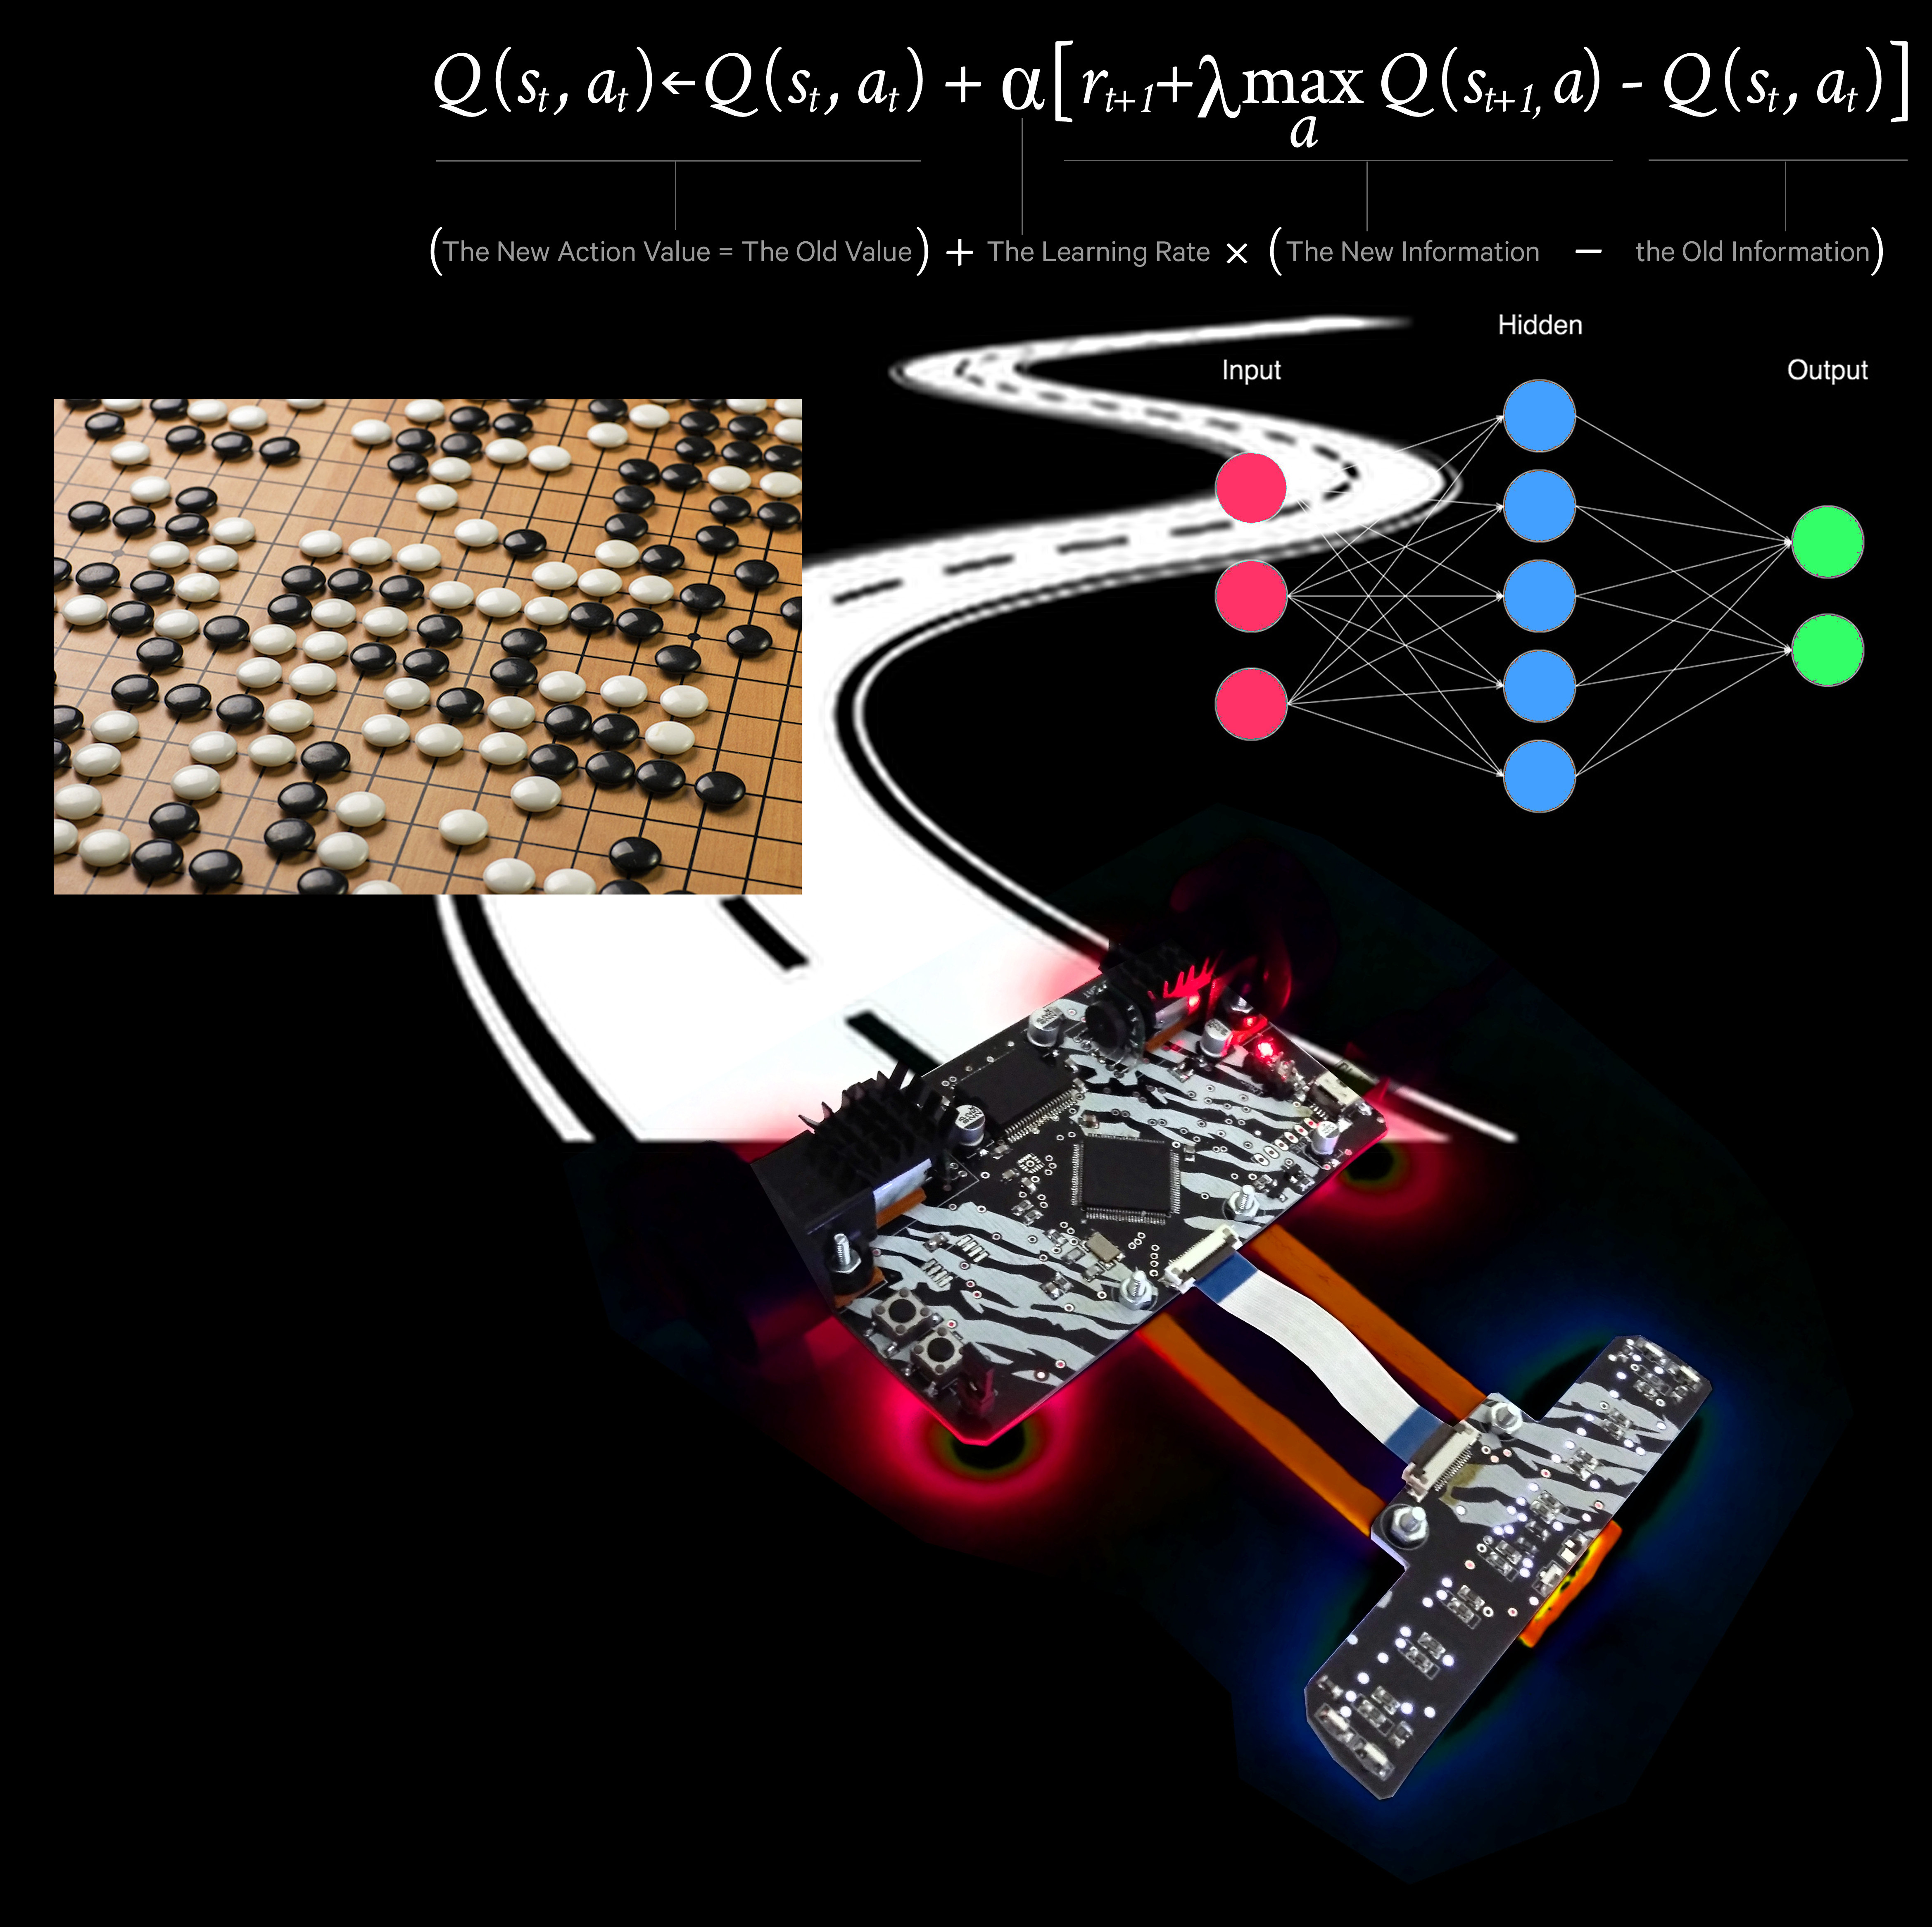
\includegraphics[width=5.05in]{./pictures/rl_square.jpg}}

        \hfil}\vfil}
    }
    \begin{frame}

    %\titlepage


    \centering
     \colorbox{black}
     {
        \begin{minipage}{7cm}
           {\LARGE \color{white} \bf Reinforcement learning} \\
           {\LARGE \color{white} Michal CHOVANEC, PhD} \\
       \end{minipage}
     }


    \end{frame}
}


\begin{frame}{\bf Reinforcement learning}

\begin{columns}
\begin{column}{0.5\textwidth}

    \centering
    \includemovie[
      poster,
      autoplay,
      externalviewer,
      inline=false,
      text={ 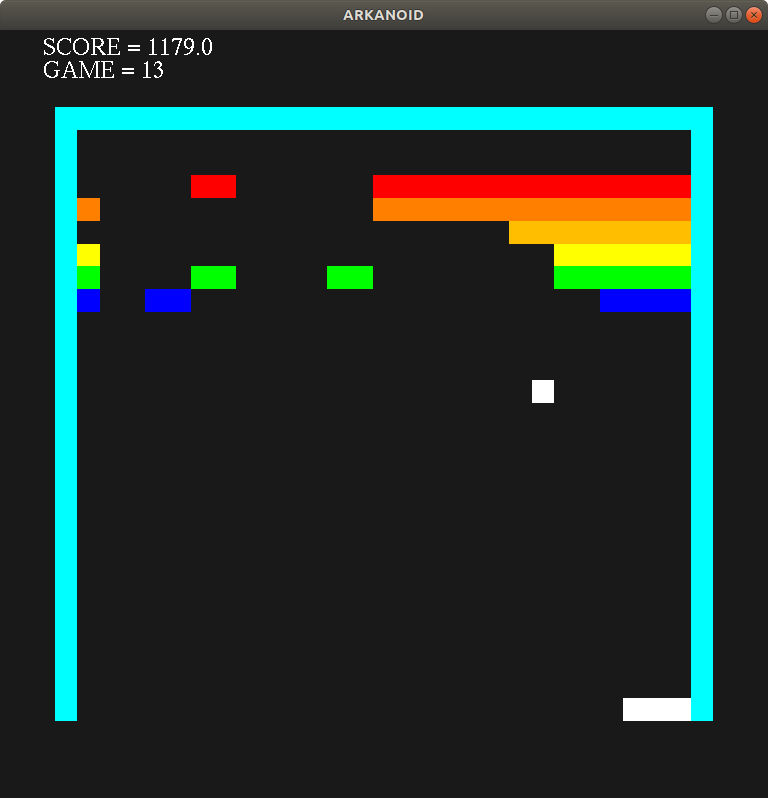
\includegraphics[scale=0.15]{./diagrams/arkanoid.png}}
    ]{4cm}{4cm}{./video/deep_reinforcement_learning_experiments.mp4}


  \begin{figure}[!htb]
    \centering
    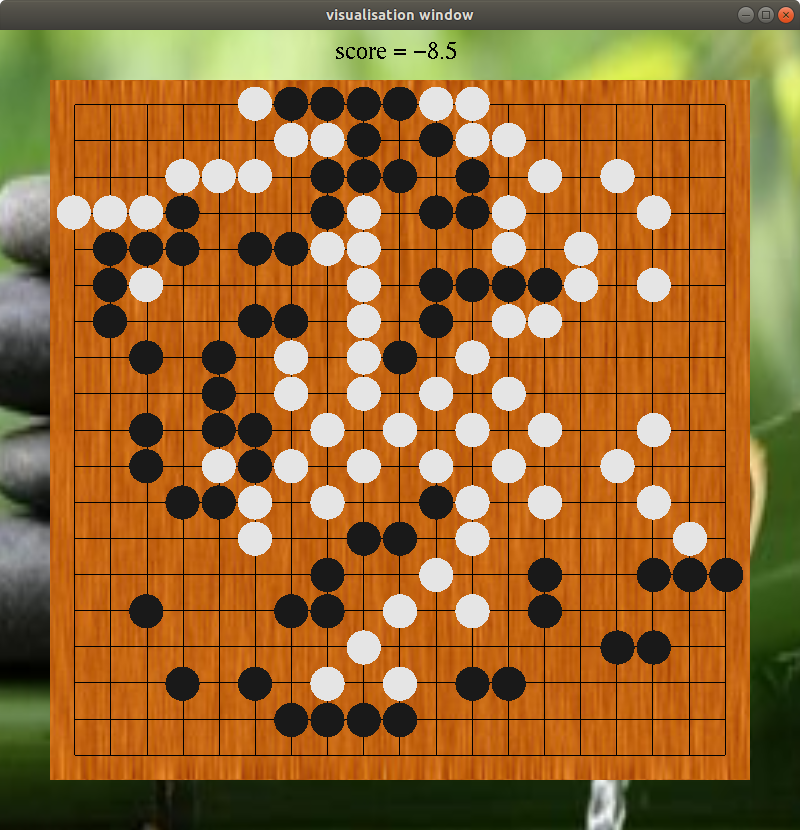
\includegraphics[scale=0.14]{./diagrams/go_board.png}
  \end{figure}


\end{column}
\begin{column}{0.5\textwidth}  %%<--- here

      \begin{itemize}
      \item {\bf playing Atari (2013)}
      \item {\bf playing GO (2016)}
      \item {\bf playing Doom (2018)}
      \item {\bf playing StarCraft (2019)}
      \item {\bf Stock market Agents, creating software, robotics}
    \end{itemize}


    \begin{figure}[!htb]
      \centering
      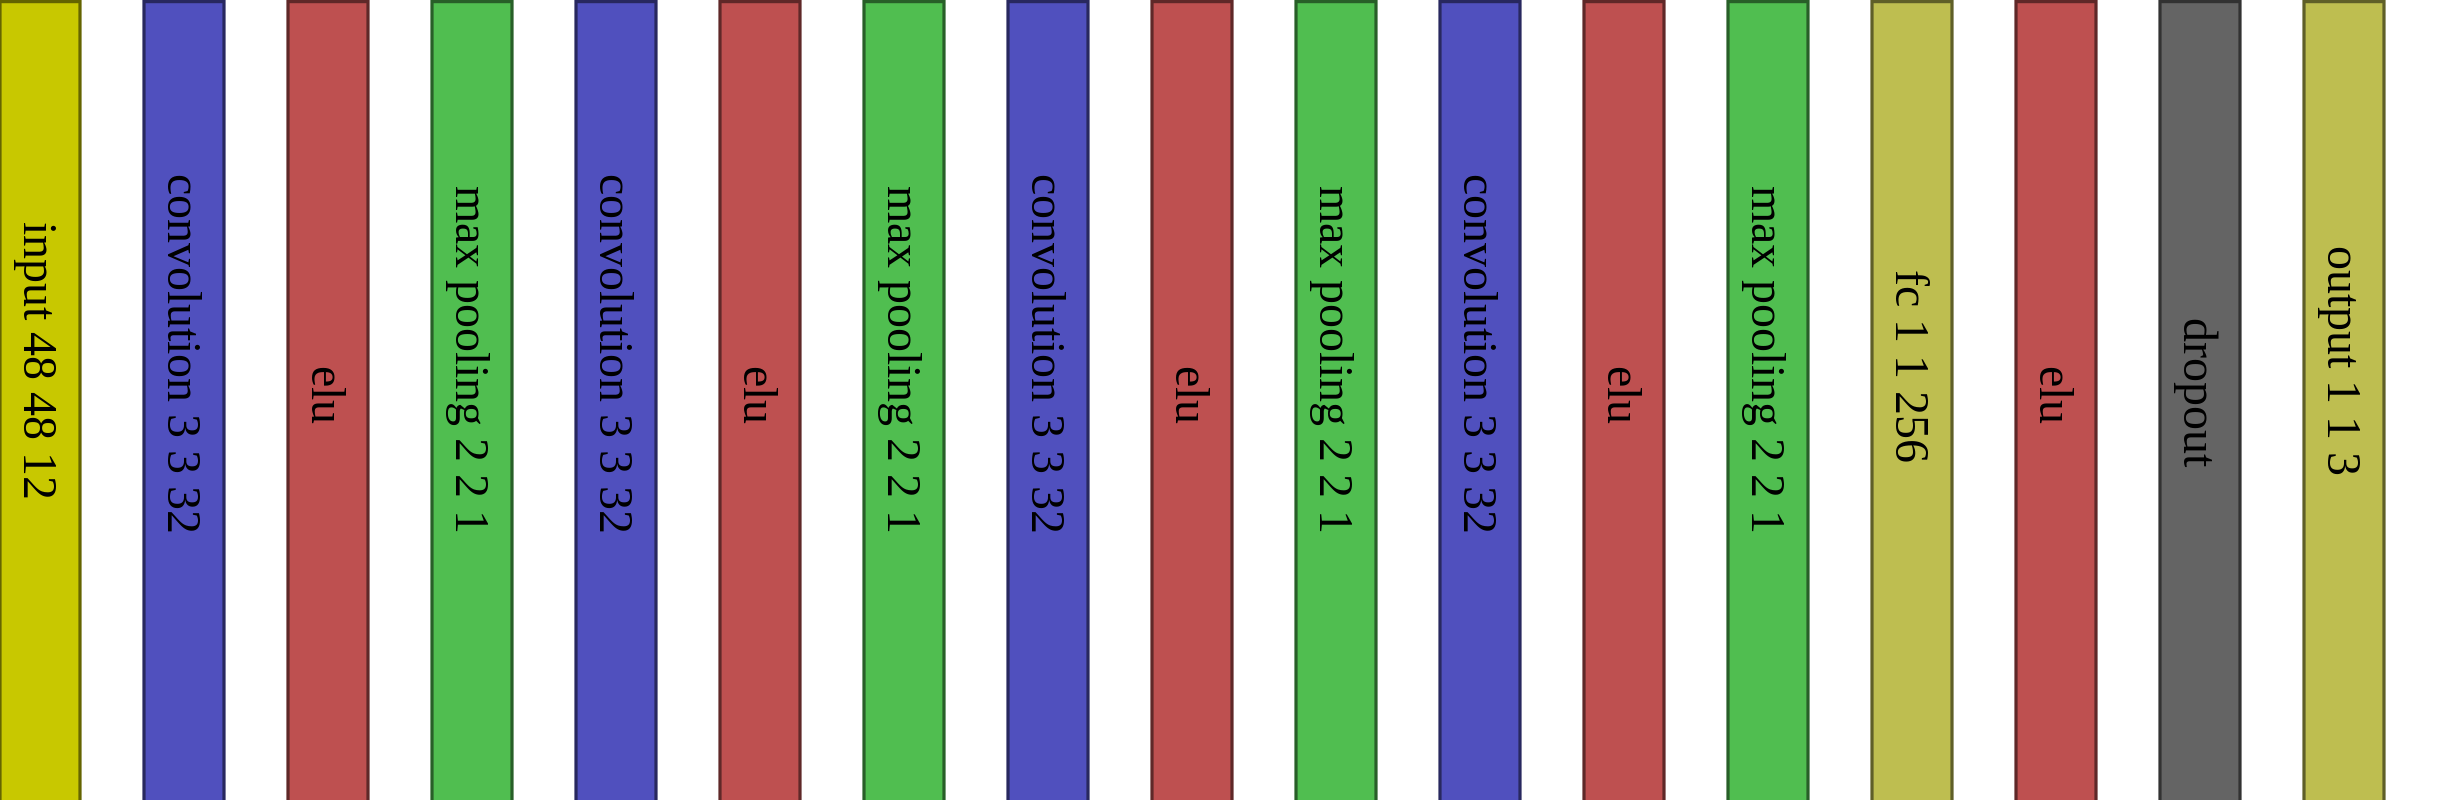
\includegraphics[scale=0.09]{./diagrams/atari_network.png}
    \end{figure}

\end{column}
\end{columns}

\end{frame}

\begin{frame}{\bf Reinforcement learning}
- learning from punishments and rewards

\begin{itemize}
  \item obtain {\bf state}
  \item choose {\bf action}
  \item {\bf execute} action
  \item obtain {\bf reward}
  \item learn from {\bf experiences}, $Q(s, a)$
\end{itemize}

  \begin{figure}
    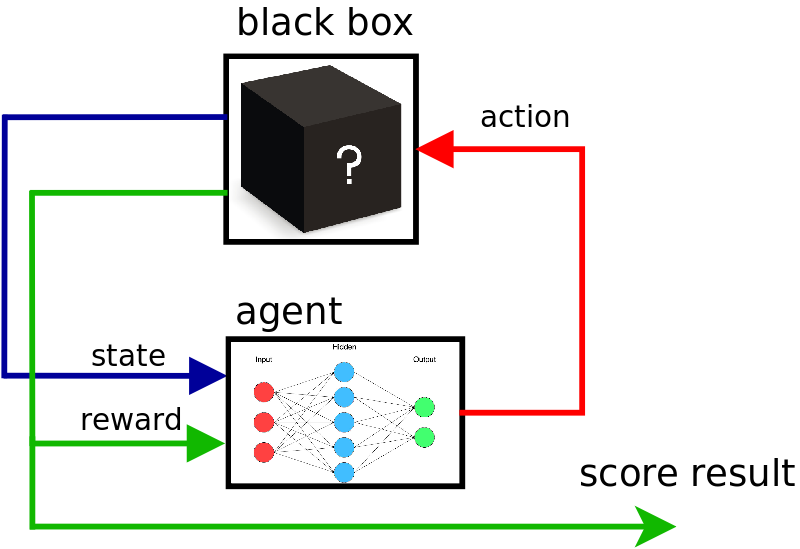
\includegraphics[scale=0.3]{./diagrams/rl_mechanism.png}
  \end{figure}

\end{frame}



\begin{frame}{\bf What is $Q(s, a)$}

Q-learning algorithm

$Q(s, a)$ value of action $a$, executed in state $s$

\begin{columns}
\begin{column}{0.5\textwidth}

  \begin{align*}
  Q(s, a) = R + \gamma \max \limits_{\alpha'} Q(s', \alpha')
  \end{align*}

\end{column}
\begin{column}{0.5\textwidth}  %%<--- here


  \begin{figure}[!htb]
    \centering
    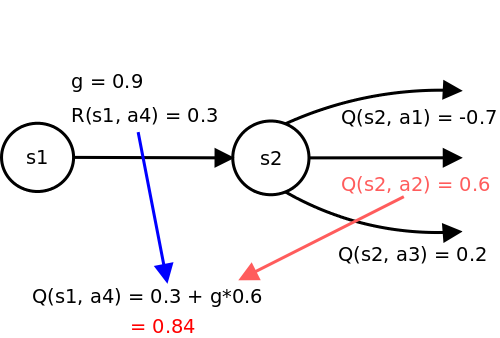
\includegraphics[scale=0.2]{./diagrams/q_learning_detail.png}
  \end{figure}

\end{column}
\end{columns}



where \\
$s$ is state \\
$a$ is action \\
$s'$ is next state \\
$a'$ is best action in next state \\
$R(s, a)$ is reward \\
$\gamma \in \langle 0, 1 \rangle$ is discount factor \\


\end{frame}


\begin{frame}{\bf Q table example}


\begin{itemize}
  \item control agent (yellow) from start to target, avoiding cliff (red)
  \item state  : one of 64 fields
  \item 4 actions, moving up, left, down, right
  \item reward : +1 on target field, -1 on cliff field
\end{itemize}



\begin{columns}
\begin{column}{0.4\textwidth}

    \begin{figure}
      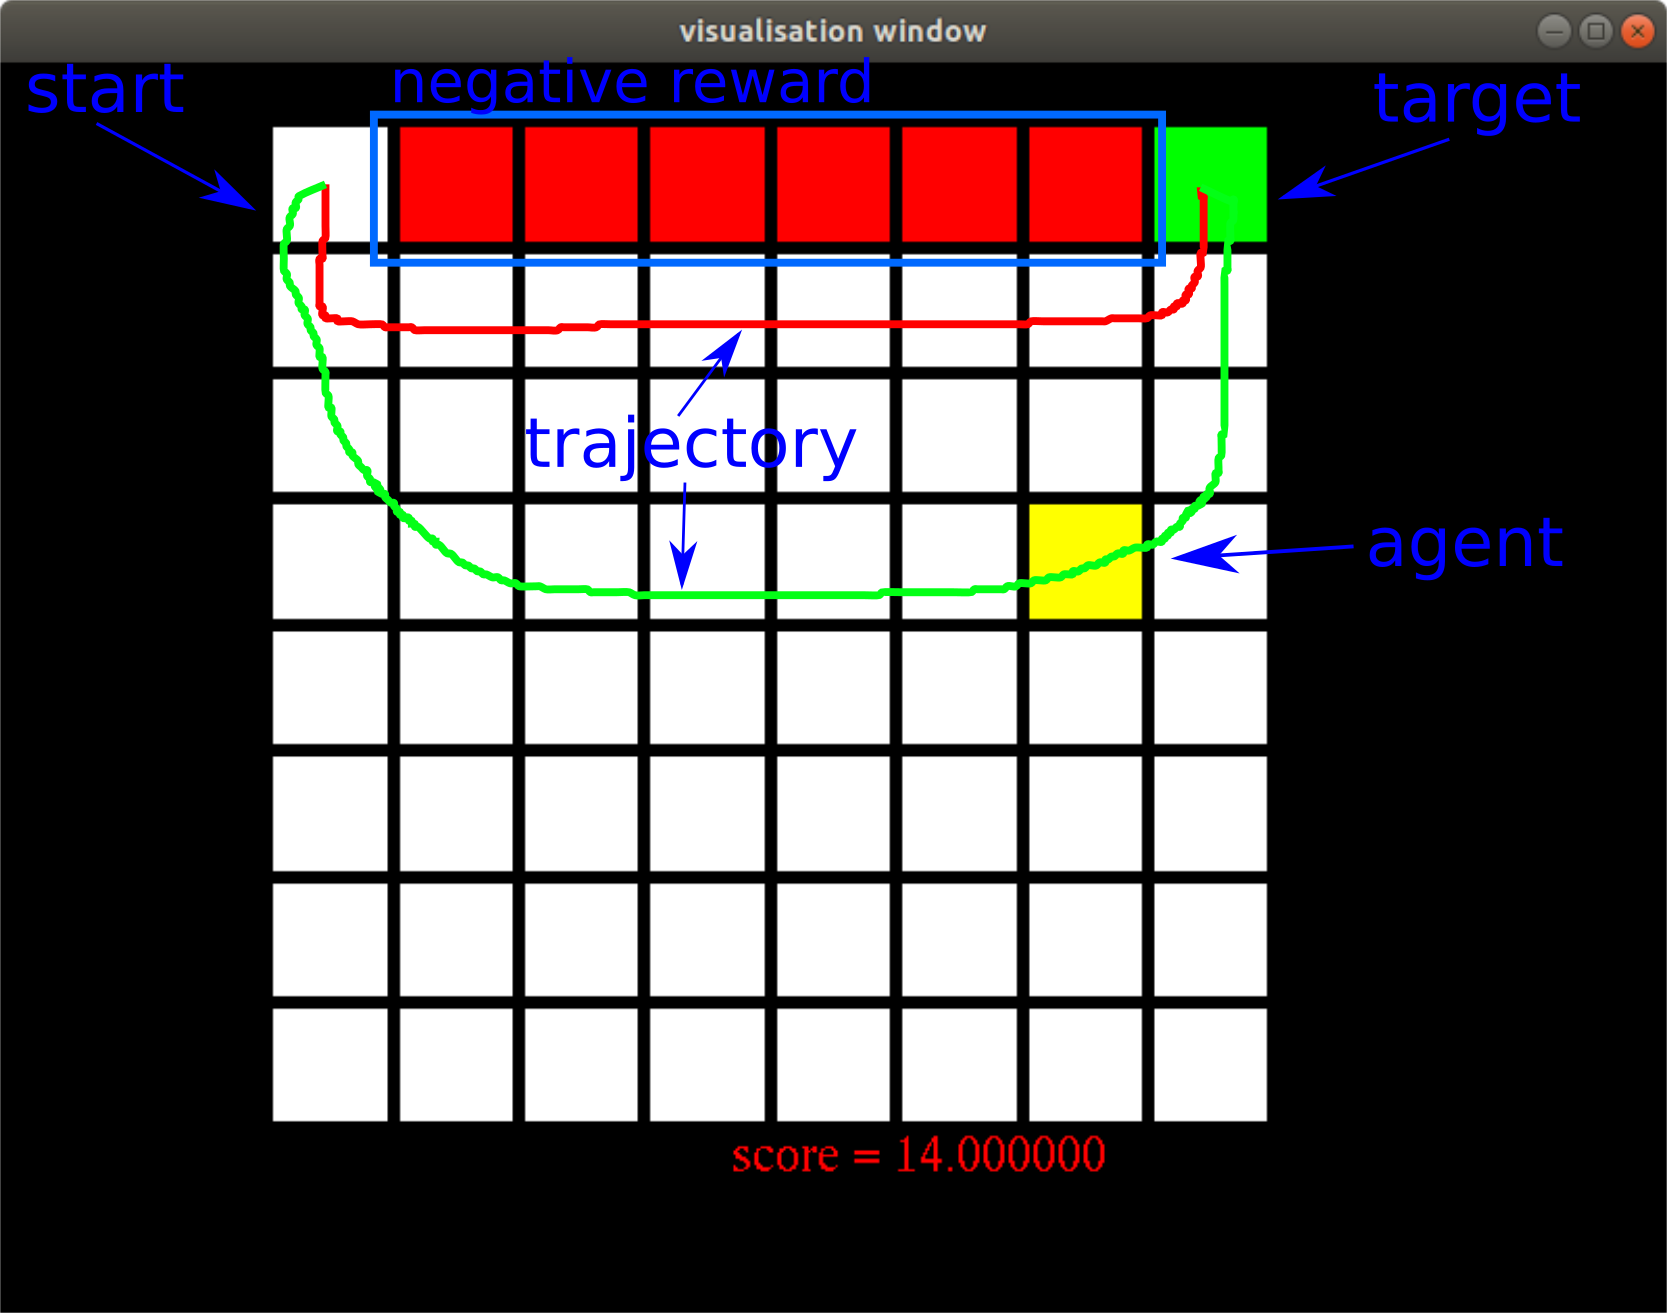
\includegraphics[scale=0.2]{./diagrams/cliff_diagram.png}
    \end{figure}


\end{column}
\begin{column}{0.5\textwidth}  %%<--- here


{\tiny
  \begin{table}[]
  \begin{tabular}{|l|l|l|l|l|}
  \hline
  \textbf{State}                                              & \textbf{UP}                    & \textbf{LEFT} & \textbf{DOWN} & \textbf{RIGHT}         \\ \hline
  0                                                           &                                   &                  & 0.43             & {\color[HTML]{FE0000} -1} \\ \hline
  \begin{tabular}[c]{@{}l@{}}1, 2, 3, \\ 4, 5, 6\end{tabular} & \textbf{T}                        & \textbf{T}       & \textbf{T}       & \textbf{T}                \\ \hline
  7                                                           & \textbf{T}                        & \textbf{T}       & \textbf{T}       & \textbf{T}                \\ \hline
  8                                                           &                                   &                  &                  & 0.49                      \\ \hline
  9                                                           & {\color[HTML]{FE0000} -1}         &                  &                  & 0.53                      \\ \hline
  10                                                          & {\color[HTML]{FE0000} -1}         &                  &                  & 0.59                      \\ \hline
  11                                                          & {\color[HTML]{FE0000} -1}         &                  &                  & 0.65                      \\ \hline
  12                                                          & {\color[HTML]{FE0000} -1}         &                  &                  & 0.72                      \\ \hline
  13                                                          & {\color[HTML]{FE0000} -1}         &                  &                  & 0.81                      \\ \hline
  14                                                          & {\color[HTML]{FE0000} -1}         &                  &                  & 0.9                       \\ \hline
  \textbf{15}                                                 & {\color[HTML]{34FF34} \textbf{1}} &                  &                  &                           \\ \hline
  \end{tabular}
  \end{table}
}

\end{column}
\end{columns}



\end{frame}



\begin{frame}[fragile]
{\bf Q table agent}

\lstset{language=python,
                basicstyle=\tiny,
                emph={self},
                emphstyle={\color{blue}},
                numberstyle=\color{green}\tiny,
                keywordstyle=\color{red}\bf\ttfamily,
                stringstyle=\color{red}\ttfamily,
                commentstyle=\color{green}
}

\begin{lstlisting}
def __init__(self):
    #get state size, and actions count
    self.states_count  = self.env.get_size()
    self.actions_count = self.env.get_actions_count()
    #init Q table, using number of states and actions
    self.q_table = numpy.zeros((self.states_count, self.actions_count))

def main(self):
    #Q learning needs to remember current state, action and previous state and action
    self.state_prev = self.state
    self.state      = self.env.get_observation().argmax()

    self.action_prev    = self.action
    #select action is done by probality selection using epsilon
    self.action         = self.select_action(self.q_table[self.state], epsilon)

    #obtain reward from environment
    reward = self.env.get_reward()

    #process Q learning
    q_tmp = self.q_table[self.state].max()

    d = reward + self.gamma*q_tmp - self.q_table[self.state_prev][self.action_prev]

    self.q_table[self.state_prev][self.action_prev]+= self.alpha*d

    #execute action
    self.env.do_action(self.action)
\end{lstlisting}


\end{frame}


\begin{frame}{\bf Deep Q network - DQN (2013)}

Approximate $Q(s, a)$ using deep neural network as $\hat{Q}(s, a; w)$, where $w$ are learnable network parameters

\begin{align*}
  Q(s, a) &= R + \gamma \max \limits_{\alpha'} Q(s', \alpha') \\
  \hat{Q}(s, a; w) &= R + \gamma \max \limits_{\alpha'} \hat{Q}(s', \alpha'; w)
\end{align*}

error to minimize
\begin{align*}
  E = \underset{\bf \color{green} target\ value}{R + \gamma \max \limits_{\alpha'} \hat{Q}(s', \alpha'; w)} - \underset{\bf \color{red} predicted\ value}{\hat{Q}(s, a; w) }
\end{align*}

weights gradient
\begin{align*}
  \Delta w = \eta E \nabla _w \hat{Q}(s, \alpha, w)
\end{align*}

This naive NN doesn't works - solution DQN

\end{frame}


\begin{frame}{\bf Naive solutuion}

\begin{figure}
  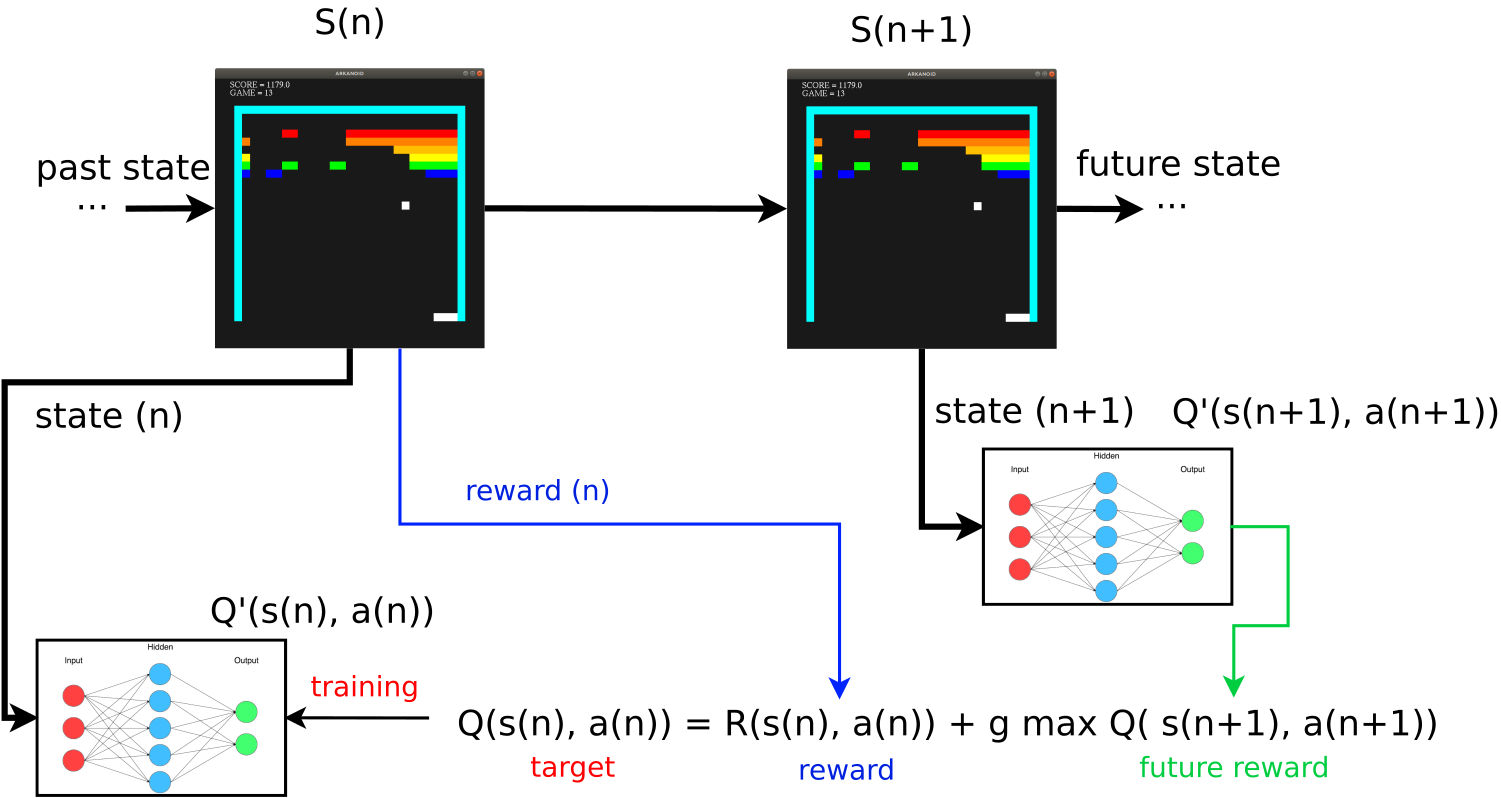
\includegraphics[scale=0.25]{./diagrams/dqn_naive.png}
\end{figure}

\end{frame}

\begin{frame}{\bf Deep Q network - DQN}

\begin{itemize}
\item {\bf \color{red} correlated states} : \\
    experience replay buffer\\
\item {\bf \color{red} unstable training} : \\
    non-stationary target value $\hat{Q}(s, a; w)$, depends on $w$, use temporary fixed weights w' \\
\item {\bf \color{red} unknow gradients values} : \\
    clip or normalise gradients into $\langle -1, 1 \rangle$
\end{itemize}
{\bf DQN equation}
\begin{align*}
  \hat{Q}(s, a; w) &= R + \gamma \max \limits_{\alpha'} \hat{Q}(s', \alpha'; w')
  \label{eq:dqn}
\end{align*}

%E &= R + \gamma \max \limits_{\alpha'} \hat{Q}(s', \alpha'; w') - \hat{Q}(s, a; w)


\begin{figure}[!htb]
  \centering
  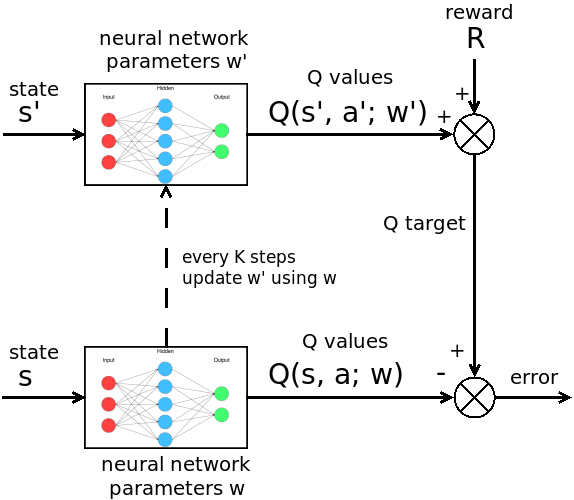
\includegraphics[scale=0.16]{./diagrams/dqn.png}
  \label{img:dqn}
\end{figure}


\end{frame}


\begin{frame}{\bf Experience replay buffer solution}

\begin{figure}
  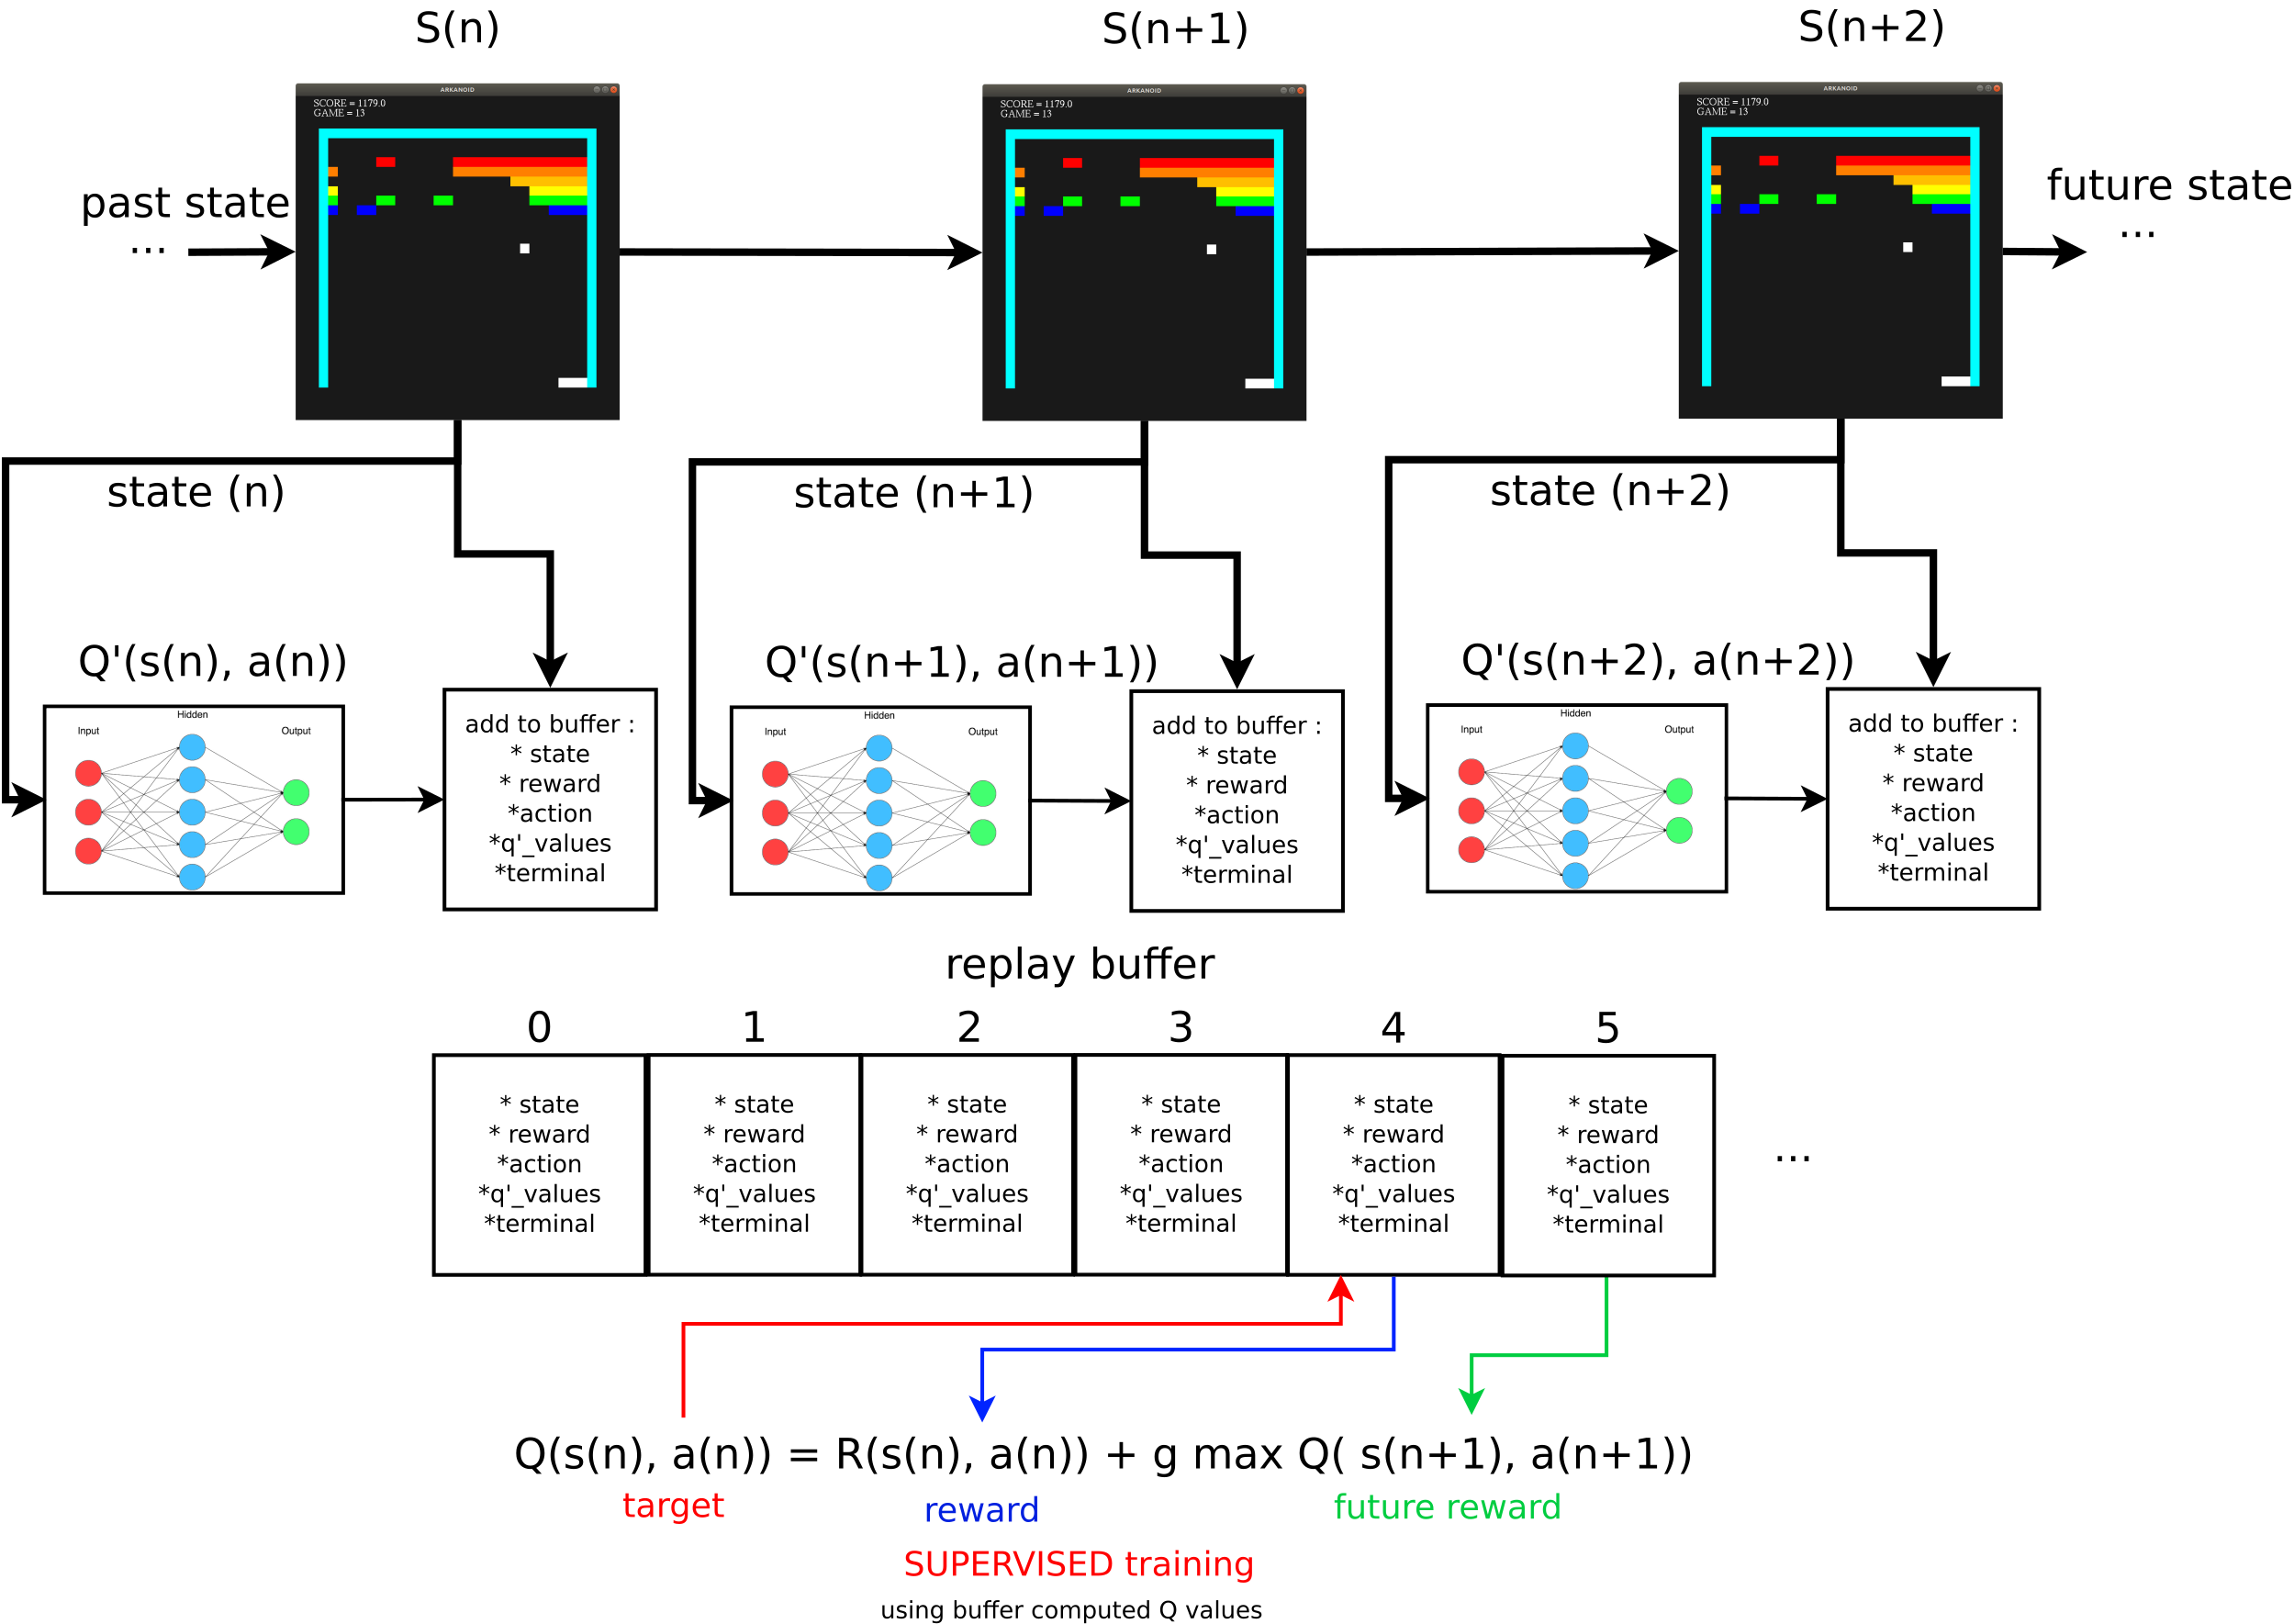
\includegraphics[scale=0.15]{./diagrams/dqn_replay_buffer.png}
\end{figure}

\end{frame}


\begin{frame}{\bf DQN best practices}
\vspace{-5mm}

{\small
\begin{itemize}
  \item {\color{red} \bf avoid} poor CNN, without FC layer, FC layer increase training speed, {\color{red} \bf avoid} global average pooling (GAP)
  \item for {\color{green} \bf short time sequence} use frame stacking, for {\color{green} \bf long time sequence} time sequences use one LSTM (GRU) layer instead of FC
  \item {\color{green} \bf use} 3x3 kernels and deeper architecture
\end{itemize}
}

{\small

    \begin{table}[]
    \begin{tabular}{|l|l|l|}
    \hline
    \textbf{layer}       & \textbf{kernel size} & \textbf{output size} \\ \hline
    \rowcolor[HTML]{C0C0C0}
    \textbf{input}       & -                    & 48x48x(3x4)          \\ \hline
    \rowcolor[HTML]{FD6864}
    \textbf{conv}        & 3x3x32               & 48x48x32             \\ \hline
    \rowcolor[HTML]{9698ED}
    \textbf{max pooling} & 2x2                  & 24x24x32             \\ \hline
    \rowcolor[HTML]{FD6864}
    \textbf{conv}        & 3x3x32               & 24x24x32             \\ \hline
    \rowcolor[HTML]{9698ED}
    \textbf{max pooling} & 2x2                  & 12x12x32             \\ \hline
    \rowcolor[HTML]{FD6864}
    \textbf{conv}        & 3x3x32               & 12x12x32             \\ \hline
    \rowcolor[HTML]{9698ED}
    \textbf{max pooling} & 2x2                  & 6x6x32               \\ \hline
    \rowcolor[HTML]{FD6864}
    \textbf{conv}        & 3x3x32               & 6x6x32               \\ \hline
    \rowcolor[HTML]{9698ED}
    \textbf{max pooling} & 2x2                  & 3x3x32               \\ \hline
    \rowcolor[HTML]{C0C0C0}
    \textbf{flatten}     &                      & 1x1x288              \\ \hline
    \rowcolor[HTML]{67FD9A}
    \textbf{fc}          & 256                  & 1x1x256              \\ \hline
    \rowcolor[HTML]{67FD9A}
    \textbf{fc}          & actions\_count       & actions\_count       \\ \hline
    \end{tabular}
    \end{table}



}

\end{frame}




\begin{frame}[fragile]
{\bf Experience replay buffer}
\lstset{language=python,
                basicstyle=\tiny,
                emph={self},
                emphstyle={\color{blue}},
                numberstyle=\color{green}\tiny,
                keywordstyle=\color{red}\bf\ttfamily,
                stringstyle=\color{red}\ttfamily,
                commentstyle=\color{green}
}

store : state, q\_values, action, reward, terminal state

\begin{lstlisting}
#init buffer
self.replay_buffer = []

#perform add at each step
def add(self):
    buffer_item  = {
        "state"        : state_vector,
        "q_values"     : q_values,
        "action"       : self.action,
        "reward"       : self.reward,
        "terminal"     : self.env.is_done()
    }
    self.replay_buffer.append(buffer_item)
\end{lstlisting}

\end{frame}




\begin{frame}[fragile]
{\bf Experience replay buffer - computing Q values}
\lstset{language=python,
                basicstyle=\tiny,
                emph={self},
                emphstyle={\color{blue}},
                numberstyle=\color{green}\tiny,
                keywordstyle=\color{red}\bf\ttfamily,
                stringstyle=\color{red}\ttfamily,
                commentstyle=\color{green}
}

\begin{lstlisting}
if self.replay_buffer.is_full():
    #compute buffer Q values, using Q learning
    for n in reversed(range(self.replay_buffer_size-1)):
        #choose zero gamme if current state is terminal
        if self.replay_buffer[n]["terminal"] == True:
            gamma = 0.0
        else:
            gamma = self.gamma

        action_id = self.replay_buffer[n]["action"]

        #Q-learning : Q(s[n], a[n]) = R[n] + gamma*max(Q(s[n+1]))
        q_next = max(self.replay_buffer[n+1]["q_values"])

        self.replay_buffer[n]["q_values"][action_id] = self.replay_buffer[n]["reward"] + gamma*max(self.replay_buffer[n+1]["q_values"])

        #clamp Q values into range <-10, 10> to prevent divergence
        for action in range(self.env.get_actions_count()):
            self.replay_buffer[n]["q_values"][action] = self.__clamp(self.replay_buffer[n]["q_values"][action], -10.0, 10.0)
\end{lstlisting}


\end{frame}




\begin{frame}[fragile]
{\bf Training CNN}

{\bf we converted reinfrocement learning problem to supervised (regression) learning problem}

\begin{itemize}
    \item replay\_buffer[n]["state"]: network input
    \item replay\_buffer[n]["q\_values"] : target values
\end{itemize}

\lstset{language=python,
                basicstyle=\tiny,
                emph={self},
                emphstyle={\color{blue}},
                numberstyle=\color{green}\tiny,
                keywordstyle=\color{red}\bf\ttfamily,
                stringstyle=\color{red}\ttfamily,
                commentstyle=\color{green}
}

\begin{lstlisting}

self.cnn.set_training_mode()

for i in range(self.replay_buffer_size):

    #choose random item, to break correlations
    idx = random.randint(0, self.replay_buffer_size - 1)

    state = self.replay_buffer[idx]["state"]
    target_q_values = self.replay_buffer[idx]["q_values"]

    #fit network
    self.cnn.train(target_q_values, state)

self.cnn.unset_training_mode()

#clear buffer
self.replay_buffer = []

\end{lstlisting}

\end{frame}




\begin{frame}{\bf Q\&A - consultations on Rysy Hut 2250 m.a.s.l.}
 \vspace{-6mm}
\begin{figure}
  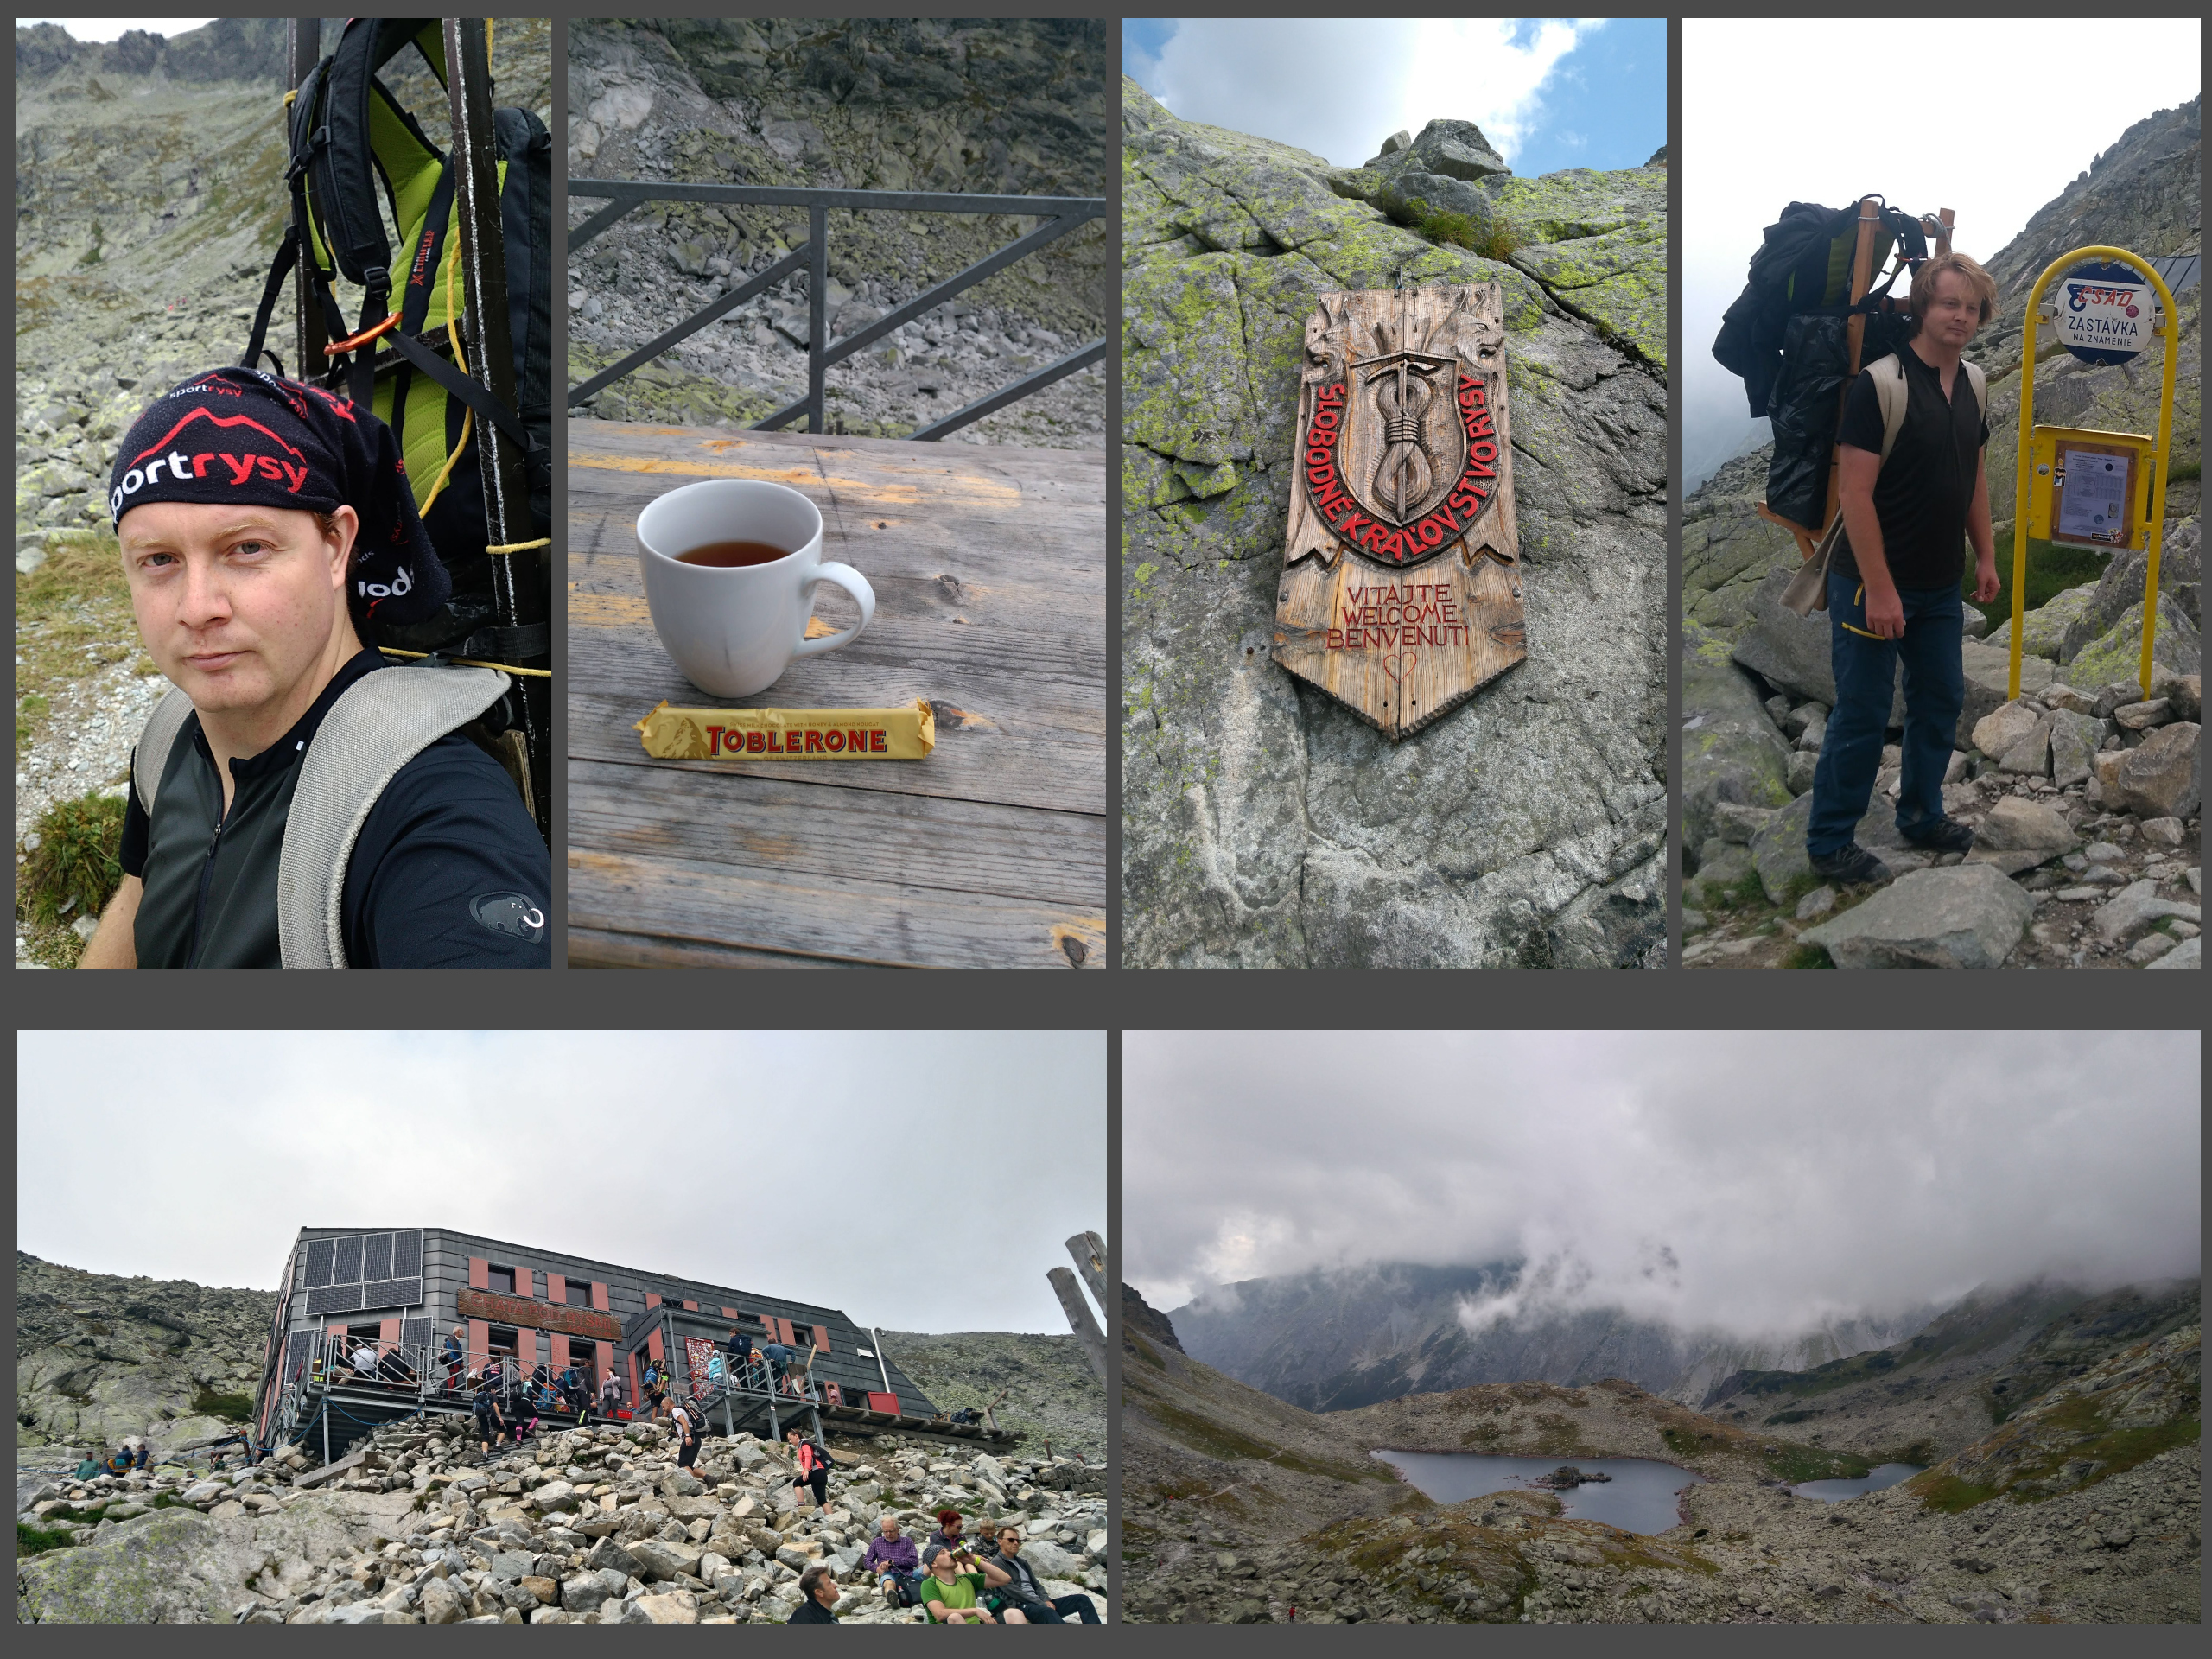
\includegraphics[scale=0.5]{./pictures/me_rysy.jpg}
\end{figure}

\end{frame}


\end{document}
